\documentclass[a4paper]{report} % estilo do documento

\usepackage[utf8]{inputenc} %encoding do ficheiro
\usepackage[portuges]{babel} % para língua portuguesa
\usepackage{graphicx} % para importar imagens
\usepackage{indentfirst}

\begin{document}

\title{Relatório Trabalho Prático LI1}
\author{Grupo 118\\
\\
Diogo Rio e  Jorge Cerqueira}
\date{\today}

\maketitle

\tableofcontents

\listoffigures

%% Introdução
\chapter{Introdução}

O objetivo deste projeto é criar em Haskell uma adaptação do clássico jogo de corridas Micro Machines. O principal objetivo do jogo é completar um percurso pré-definido no menor tempo possível. Este percurso pode ter diferentes alturas e é rodeado por lava.O jogador é penalisado sempre que sofre uma queda dentro do percurso ou cai na lava.
No âmbito de melhor resolver este problema, este projeto foi dividido em duas fazes que serão analisadas no decorrer deste relatório.

%% Análise de Requisitos e Especificação do Problema
\chapter{Análise de Requisitos}


\section{Fase 1}
\label{sec:analisefase1}

O objetivo desta fase é a criação de todas as funções que serão necessárias para o funcionamento do jogo propriamente dito (esqueleto do jogo), tais como funções para criação de mapas, validação de mapas, e funções necessárias para a movimentação do carro no mapa de jogo e as respectivas colisões com obstáculos.


\section{Fase 2}
\label{sec:analisefasee}

O objetivo desta fase do projecto será criar o jogo propriamente dito, ou seja, a criação de funções para input do utilizador, funções para a atualização do estado do jogo, criação de menus, scoreboard's etc. Será também um objetivo desta fase a criação de um bot que jogue o jogo automaticamente.

%% Descrição da Solução Desenvolvida
\chapter{A Nossa Solução}

Para a melhor compreenção do leitor esta fase estará em 3 subfases.

\subsection{Construção de mapas}

Nesta primeira subfase o principal objetivo será a elaboração de uma função que construa um mapa para o jogo seguindo um caminho previamente registado, caminho este que consiste numa lista de passos, onde cada passo é
uma das seguintes opções: avança, sobe, desce , curva à esquerda ou curva à direita.
Esta função será a função constroi :

\begin{verbatim}
constroi :: Caminho -> Mapa
constroi c = Mapa (partida c,Este) (makeTabuleiro c)
\end{verbatim}
A principal parte de esta função é a função makeTabuleiro :

\begin{verbatim}
makeTabuleiro :: Caminho -> Tabuleiro
makeTabuleiro steps = 
makeTabuleiroH (reverse(makePath steps)) (tabuleiroInit (dimensao steps))
    where
     makeTabuleiroH [] ac = ac
     makeTabuleiroH (step:steps) ac = makeTabuleiroH steps (swapTabuleiroPeca ac peca pos)
                                       where (peca,pos) = step
\end{verbatim}
que dado um caminho devolve um tabuleiro que contem as peças obtidas na função makePath-foi aplicada a função reverse (que reverte uma lista) a esta função uma vez que a lista proveniente estava ao contrário-e onde as restantes peças são do tipo lava.






A função makePath :

\begin{verbatim}
makePath :: Caminho -> [(Peca,Posicao)]
makePath steps = 
makePathAc (startPos,Este,0) steps []
 where
  startPos = partida steps
  makePathAc _ [] l = l
  makePathAc (pos,ori,alt) (step:steps) l = 
   makePathAc (nextPos,nextOri,nextAlt) steps ((peca,pos):l)
            where (peca,(nextPos,nextOri,nextAlt)) = nextStep (pos,ori,alt) step
\end{verbatim}
que dado um caminho devolve a lista de peças que o compoêm bem como a sua posição.Para a construção desta função é utilizada a função nextStep :

\begin{verbatim}
nextStep :: (Posicao,Orientacao,Altura) -> Passo -> (Peca,(Posicao,Orientacao,Altura))
nextStep ((x,y),ori,alt) Avanca   = 
( Peca  Recta alt,((move (x,y) ori),ori,alt))
nextStep ((x,y),ori,alt) Sobe     = 
((Peca (Rampa ori) alt),((move (x,y) ori),ori,alt+1))
nextStep ((x,y),ori,alt) Desce    = 
((Peca (Rampa (invertOri ori)) (alt-1)),((move (x,y) ori),ori,alt-1))
nextStep ((x,y),ori,alt) CurvaDir = 
((Peca (Curva ori) alt),((move (x,y) (rodaOriDir ori)),(rodaOriDir ori),alt))
nextStep ((x,y),ori,alt) CurvaEsq = 
((Peca (Curva (rodaOriDir ori)) alt),((move (x,y) (rodaOriEsq ori)),(rodaOriEsq ori),alt))
\end{verbatim}
que devolve a peça correspondente a uma certa posição, orientação e altura, assim como a posição,orientação e altura da peça seguinte dado um certo passo.Esta função utiliza funções como a função move-que dada uma poisção e uma orientação devolve uma nova posição que é a posição movida para cima, baixo, esquerda ou direita dependendo a orientação-,rodaOriDir, RodaOriEsq e invertOri que rodam uma orientação 90º para a direita, esquerda e que inverte em 180º uma orientação, respetivamente.


\section{Fase 1}

\subsection{Validação do Mapa}
O objetivo desta subfase é a criação de uma função para a validação de um mapa, ou seja, para averiguar se um determinado mapa segue um conjunto de regras para que possa ser utilizado no nosso jogo , a saber :

\begin{itemize}
    \item Existe apenas um percurso e todas as peças fora desse percurso são do tipo lava
    \item O percurso deve corresponder a uma trajetória, tal que começando na peça de partida com a orientação inicial se volte a chegar à peça de partida com orientação inicial.
    \item A orientação inicial tem de ser compatível com a peça de partida.
    \item As peças do percurso só podem estar ligadas a peças do percurso com alturas compatíveis.
    \item Todas as peças do tipo lava estão à altura 0.
    \item O mapa é sempre retangular e rodeado por lava.
\end{itemize}

A função final é a função valida :
\begin{verbatim}
valida :: Mapa -> Bool
valida m = 
check3 m && check5 m && check6 m && checkPassos m && checkPartida m && checkDim m
\end{verbatim}
que é a combinação de diferentes funções.
Para validar a primeira regra e a quarta regra, optamos por fazer uma função que teste se é possível converter um determinado mapa em uma lista de passos, assegurando assim que apenas existe um percurso e que todas as peças fora desse percurso são do tipo lava e que as peças do percurso estao ligadas a peças com alturas compatíveis.
Esta função é a função checkPassos :

\begin{verbatim}
checkPassos :: Mapa -> Bool
checkPassos m = 
checkPassosH (reverseMapa m) []
    where
     reverseMapa (Mapa (pos,ori) tab) = reversePassos tab pos ori
     checkPassosH [] n = (countNotLava (constroi n)) == countNotLava m
     checkPassosH (x:xs) n |x== Nothing = False
                           |otherwise   = checkPassosH xs (n++[x_])
                           where
                             Just x_ = x
\end{verbatim}
Para validar a terceira regra, é utilizada a função check3:

\begin{verbatim}
check3 :: Mapa -> Bool
check3 (Mapa (pos,ori) tab) = compativel (getPeca tab pos) ori
\end{verbatim}
onde é usada a função compativel :

\begin{verbatim}
compativel :: Peca -> Orientacao -> Bool
compativel (Peca Recta h) _ = True
compativel (Peca (Rampa ori) h) o |ori == o           = True
                                  |invertOri ori == o = True
                                  |otherwise = False

compativel (Peca Lava h) _ = False
compativel (Peca (Curva ori) h) o |ori == o||(ori == rodaOriDir o)=True
                                  |otherwise = False
\end{verbatim}
que testa se uma determinada peça é compatível com uma orientação qualquer retornando um bool, neste caso, pretendemos testar se a peça inicial é compatível com a orientação inicial, esta orientação inicial é dada no mapa e para ir buscar esta peça inicial é utilizada a função getPeca :

\begin{verbatim}
getPeca :: Tabuleiro -> Posicao -> Peca
getPeca t pos = getPecaH t pos
               where
                getPecaH2 (t:ts) 0 = t
                getPecaH2 (t:ts) x = getPecaH2 ts (x-1)
                getPecaH (t:ts) (x,0) = getPecaH2 t x
                getPecaH (t:ts) (x,y) = getPecaH (ts) (x,y-1)
\end{verbatim} 
que dada um posição e um tabuleiro devolve a respetiva peça.
Para validar a quinta regra, é utilizada a função check5:

\begin{verbatim}
check5 :: Mapa -> Bool
check5 (Mapa q [[]]) = True
check5 (Mapa q (((Peca Lava 0):xs):ys) ) = 
check5 (Mapa q (xs:ys))
check5 (Mapa q (((Peca Lava _):xs):ys) ) = False
check5 (Mapa q ([]:ys)) = check5 (Mapa q ys)
check5 (Mapa q ((x:xs):ys) ) = check5 (Mapa q (xs:ys))
\end{verbatim}
que corre todas as peças do mapa e testa se a sua altura é 0, retornando um bool no final.
Por último, para validar a ultima regra, é utilizada a função check6
\begin{verbatim}
check6 :: Mapa -> Bool
check6 (Mapa (_,_) (y:ys)) = 
check6H  y ys
 where
  check6H y [] = checkIfLava y True
  check6H y (y1:ys) |checkIfLava y False = check6H y1 ys
                    |otherwise = False
\end{verbatim}
que, aliada à função checkIfLava :

\begin{verbatim}
checkIfLava :: [Peca] -> Bool -> Bool
checkIfLava [] _ = True
checkIfLava (x:xs) True |x==l = checkIfLava xs True
                        |otherwise = False
                          where l = (Peca Lava 0)
checkIfLava (x:xs) False = checkIfLava (x:[last (x:xs)]) True
\end{verbatim} 
testa se a primeira e última lista do mapa são do tipo lava, assim como se o primeiro e ultimo elemento das restantes listas do mapa são do tipo lava, assegurando assim que o mapa é rodeado por lava.
Para assegurar que o mapa é retangular, é utilizada a função checkDim :

\begin{verbatim}
checkDim :: Mapa -> Bool
checkDim (Mapa _ (x:xs)) = 
checkDimH (length x) xs
  where
  checkDimH len [] = True
  checkDimH len (x:xs)|len == length x = checkDimH len xs
                      |otherwise = False
\end{verbatim}
que retorna um bool indicando se o mapa é ou não retangular.






\subsection{Movimentar o Carro}
O objetivo desta tarefa é começar a implementar a mecânica do jogo, nomeadamente as movimentações do carro no mapa de jogo e as respetivas colisões com obstáculos, ou seja, é necessário criar uma função que dado o estado atual de um carro calcule o seu novo estado após um determinado período de tempo.
A resolução que encontramos para este problema foi a função movimenta :

\begin{verbatim}
movimenta :: Tabuleiro -> Tempo -> Carro -> Maybe Carro
movimenta tab t c = nC
          where
          (tab_,t_,p_,nC) = moverCarro (tab,t,p,Just c)
          p = getPecaCarro (tab,Just c)
\end{verbatim}
que recebe um tabuleiro, um tempo e um carro e devolve um Maybe Carro, ou seja, devolve o novo estado do carro ou devolve "nothing" quando o carro é destruido.


Antes de mais gostaria de realçar que no decorrer da explicação desta funções irão ser usadas funções como a função add, mult, módulo e dotProduct, que são funções que fazem a soma de vetores, a multiplicação de um número por um vetor, o módulo de um vetor e o produto de dois vetors respetivamente.


A função movimenta é formada pela função moverCarro que recebe um tabuleiro, um tempo, uma peça , uma posição e um Maybe Carro.
Para a construção desta função são utilizadas outras funções auxiliares. As funções isRampa e isCurva testam se a peça que o carro está é uma rampa ou uma curva respetivamente devolvendo um bool. A função validaCurva :

\begin{verbatim}
validaCurva :: Peca -> Maybe Carro -> Bool
validaCurva (Peca (Curva Norte) h) c = y_ >= (-x_ + 1)
                                     where
                                     Just (Carro (x,y) o (vx,vy)) = c
                                     x_ = x - fromIntegral (floor x)
                                     y_ = y - fromIntegral (floor y)
validaCurva (Peca (Curva Sul)  h) c = y_ <= (-x_ + 1)
                                     where
                                     Just (Carro (x,y) o (vx,vy)) = c
                                     x_ = x - fromIntegral (floor x)
                                     y_ = y - fromIntegral (floor y)

validaCurva (Peca (Curva Este) h) c = y_ >= x_
                                     where
                                     Just (Carro (x,y) o (vx,vy)) = c
                                     x_ = x - fromIntegral (floor x)
                                     y_ = y - fromIntegral (floor y)

validaCurva (Peca (Curva Oeste) h) c = y_ <= x_
                                     where
                                     Just (Carro (x,y) o (vx,vy)) = c
                                     x_ = x - fromIntegral (floor x)
                                     y_ = y - fromIntegral (floor y)
\end{verbatim}
verifica se o carro está numa posição válida da curva, ou seja, não se encontra na parte com Lava.A função reflectCurva : 

\begin{verbatim}
reflectCurva :: Peca -> Maybe Carro -> Maybe Carro
reflectCurva (Peca (Curva o) h) c |o==Norte || o==Sul   = reflectCurvaNS c
                                  |o==Este  || o==Oeste = reflectCurvaEO c
\end{verbatim}
que reflete uma velocidade em relação ao tipo de curva, onde são utilizadas duas outras funções, a reflectCurvaNS e reflectCurvaEO que refletem a velocidade de uma curva com orientação Norte ou Sul e Este ou Oeste respetivamente :

\begin{verbatim}
reflectCurvaNS :: Maybe Carro -> Maybe Carro
reflectCurvaNS c =Just (Carro pos ori nVel)
                 where
                 Just (Carro pos ori vel) = c
                 normal = (sqrt(2)/2,sqrt(2)/2)
                 dP = dotProduct vel normal
                 nVel = add vel (mult normal ((-2)*dP))

reflectCurvaEO :: Maybe Carro -> Maybe Carro
reflectCurvaEO c =Just (Carro pos ori nVel)
                where
                Just (Carro pos ori vel) = c
                normal = (-sqrt(2)/2,sqrt(2)/2)
                dP = dotProduct vel normal
                nVel = add vel (mult normal ((-2)*dP))

\end{verbatim}
A função reflect:

\begin{verbatim}
reflect :: Posicao -> Posicao -> Maybe Carro -> Maybe Carro
reflect (xi,yi) (xf,yf) c |xi /= xf && yi /= yf = Just (Carro pos ang (-vx,-vy))
                          |xi /= xf = Just (Carro pos ang (-vx,vy))
                          |yi /= yf = Just (Carro pos ang (vx,-vy))
                          where
                          Just (Carro pos ang (vx,vy)) = c
\end{verbatim}
que inverte a velocidade do carro no eixo do x ou y. A função moverLinhaRecta que move o carro uma pequena distância em uma linha reta:

\begin{verbatim}
moverLinhaReta :: (Tempo,Maybe Carro) -> (Tempo,Maybe Carro)
moverLinhaReta (t,c) |t<=0 = (0,moverTempo t c)
                     |otherwise = (nT,moverTempo t_ c)
                     where
                     Just (Carro pos ang vel) = c
                     nT = t-t_
                     t_ = 0.05/(modulo vel)
\end{verbatim}
que utiliza a função moverTempo que dado um tempo e um carro devolve o carro quando aplicada a velocidade no espaço de tempo dado :

\begin{verbatim}
moverTempo :: Tempo -> Maybe Carro -> Maybe Carro
moverTempo t c = nC
               where
               Just (Carro pos ang vel) = c
               nPos = add pos (mult vel t)
               nC = Just (Carro nPos ang vel)
\end{verbatim}
E por último a função getPecaCarro que devolve a peça em que se encontra o carro :

\begin{verbatim}
getPecaCarro :: (Tabuleiro,Maybe Carro) -> (Peca,Posicao)
getPecaCarro (t,c) = ((t !! y_) !! x_,(x_,y_))
                where
                Just (Carro (x,y) ang (vx,vy)) = c
                x_ = floor x
                y_ = floor y
\end{verbatim}



\section{Fase 2}

Iremos também dividir esta fase em 3 subfase para melhor compreensão do leitor.

\subsection{Atualizar Estado}

De modo a melhor resolver os problemas desta subfase decidimos que seria melhor criar uma libraria ("VectorLib") onde foram feitas funções simples para operações com vetores, por exemplo, soma de vetores, multiplicação de vetores, etc.

O objetivo desta subfase é atualizar o estado do jogo dadas as ações efectuadas por um jogador num período de tempo. Para tal, é necessário criar o estado interno do jogo que atualize a cada instante (Jogo) e funções de input do jogador (Acao).

O estado do jogo em cada momento é definido por um mapa e as propriedades desse mapa, e, para cada um dos jogadores, o estado do carro, a quantidade de “nitro” disponível e o histórico de todas as posições visitadas.

A nossa solução para o problema é a função atualiza :

\begin{verbatim}
atualiza :: Tempo -- ^ a duração da ação
         -> Jogo  -- ^ o estado do jogo
         -> Int   -- ^ o identificador do jogador
         -> Acao  -- ^ a ação tomada pelo jogador
         -> Jogo  -- ^ o estado atualizado do jogo
atualiza t (Jogo map pist cars nits hists) j a
  = (Jogo map pist nCars nNits nHists)
  where
  car  = cars !! j
  nit  = nits !! j
  hist = hists !! j
  aReceberNitro = lNitros !! j
  lNitros = calcularNitros a nits (replicate (length nits) False)
  (nCar,nNit,nHist) = updateCarro map pist a car nit t hist aReceberNitro
  (nCars,nNits,nHists) = (swapAt j nCar cars,
                          swapAt j nNit nits,
                          swapAt j nHist hists
                          )
\end{verbatim}
onde usamos a função updateCarro para atualizar a posição e a velocidade de um carro :

\begin{verbatim}
updateCarro :: Mapa -> Propriedades -> Acao -> Carro -> Tempo -> Tempo -> [Posicao]
               -> Bool -- Verifica se o carro está a receber nitro
               -> (Carro, Tempo, [Posicao])
updateCarro m p a c tNitro tStep hist n
  = ((Carro (x,y) nDirecao novaVel), nTNitro, nListaPos)
  where
  Propriedades atr pen ace pes nit rod = p
  (Carro (x,y) ang vel) = c
  novaVel     = vAdd vel somaForcas
  somaForcas  = (vAddList [fAtrito,fAcelaracao,fGravidade,fPneus,fNitro])
  fAtrito     = calcularAtrito atr c tStep
  fAcelaracao = calcularAceleracao a c ace tStep
  fGravidade  = calcularPeso m c pes tStep
  fPneus      = calcularFPneus c pen tStep
  fNitro      = calcularFNitro c n nit tStep
  nDirecao    = calcularAngulo a c rod tStep
  nTNitro     = calculaTempoNitro a tNitro tStep
  posicao     = (floor x,floor y)
  nListaPos   = addToLista posicao hist
\end{verbatim}
Na função acima, para calcular a velocidade do carro são necessárias funções que calculem as forças aplicadas no carro face às propriedades do mapa, comecemos então pela função calcularAtrito :

\begin{verbatim}
calcularAtrito :: Double -> Carro -> Tempo -> Vetor
calcularAtrito a (Carro _ _ v) t 
  = vMult v (-a/1*t)
\end{verbatim}
que devolve a força aplicada pelo atrito, a função calcularAngulo :

\begin{verbatim}
calcularAngulo :: Acao -> Carro -> Double -> Tempo -> Angulo
calcularAngulo (Acao _ _ kE  kD  _) (Carro _ a _) rod t
  = case (kE,kD) of
    (True,False) -> a + (rod*t)
    (False,True) -> a - (rod*t)
    otherwise    -> a
\end{verbatim}
que devolve o novo ângulo para o qual o carro está virado, a função calcularAcelaração :

\begin{verbatim}
calcularAceleracao :: Acao -> Carro -> Double -> Tempo -> Vetor
calcularAceleracao (Acao kA kT _ _ _) (Carro _ a v) ace t
  = case (kA,kT) of
    (True,False) -> vMult (vFromAngle (-a*pi/180)) (ace*t)
    (False,True) -> vMult (vFromAngle (-a*pi/180)) (-ace*t)
    otherwise    -> (0,0)
\end{verbatim}
que devolve a força exercida pela aceleração do carro, a função calcularFPeneus : 

\begin{verbatim}
calcularFPneus :: Carro -> Double -> Tempo -> Vetor
calcularFPneus (Carro _ a (0,0)) _ _ = (0,0)
calcularFPneus (Carro _ a v) pen t
  |vDot fPneus v > 0 = vMult fPneus (-norma*t)
  |otherwise         = vMult fPneus (norma*t)
  where
  fPneus = vPerpendicularFromAng (vDegreeToRad (-a))
  norma  = (sin ang) * pen * (vMag v)
  ang    = vAngleBetween v aVetor
  aVetor = vFromAngle (-a*pi/180)
\end{verbatim}
que devolve a força exercida pelos pneus do carro numa curva, a função calcularFNitro : 

\begin{verbatim}
calcularFNitro :: Carro -> Bool -> Double -> Tempo -> Vetor
calcularFNitro _ False _ _
  = (0,0)
calcularFNitro (Carro _ ang _) True nit t
  = let vec = vFromAngle (vDegreeToRad (-ang)) in
    vSetMag (nit*t) vec
\end{verbatim}
que calcula a força do nitro aplicada a um carro e por último a função calcularPeso

\begin{verbatim}
calcularPeso :: Mapa -> Carro -> Double -> Tempo -> Vetor
calcularPeso (Mapa _ tab) (Carro (x,y) _ _) grav t
  = vMult peso t
  where
  --Função que calcula o peso do carro
  peso = vMult (pecaToVet peca) grav
  peca = obterPeca (floor x, floor y) tab
\end{verbatim}
que calcula o peso que está a ser aplicado no carro e usa como função auxiliar as funções obterPeca e pecaToVet :

\begin{verbatim}
obterPeca (x,y) tab = ((tab !! y) !! x)
\end{verbatim}

\begin{verbatim}
pecaToVet :: Peca -> Vetor 
  pecaToVet (Peca (Rampa o) _)
    = gravOri o
    where
    gravOri Sul   = ( 0,-1)
    gravOri Norte = ( 0, 1)
    gravOri Este  = (-1, 0)
    gravOri Oeste = ( 1, 0)
  pecaToVet _ = (0,0)
\end{verbatim}
que devolve a peça em que o carro se encontra e devolve o vetor normalizado da gravidade para uma certa peça respetivamente.

É usada também na função updateCarro a função addToLista : 

\begin{verbatim}
addToLista :: Posicao -> [Posicao] -> [Posicao]
addToLista (a,b) [] = [(a,b)]
addToLista pos1 xxs@(pos2:_)
  |pos1 == pos2 = xxs
  |otherwise    = pos1:xxs
\end{verbatim}
que é a função que adiciona uma posicao a uma lista de posicões se a cabeça desta for diferente
à posição a adicionar.


Para resolver a questão dos nitros, usamos as funções calcularNitros : 

\begin{verbatim}
calcularNitros :: Acao -> [Tempo] -> [Bool] -> [Bool]
calcularNitros a [] b = b
calcularNitros a (t:ts) b
  = calcularNitros a ts nB
  where
  nB = nitroToBool a t b
\end{verbatim}
que calcula os carros que estão a receber nitro e usa a função nitroToBool como auxiliar :

\begin{verbatim}
nitroToBool :: Acao ->  Tempo -> [Bool] -> [Bool]
nitroToBool _ 0 bools = bools
nitroToBool (Acao _ _ _ _ Nothing) _ bools = bools
nitroToBool (Acao _ _ _ _ (Just n)) _ bools
  = nitroToBoolH 0 n bools
  where
  nitroToBoolH x n [] = []
  nitroToBoolH x n (bool:bools)
    |x==n = True : bools
    |otherwise = bool : (nitroToBoolH (x+1) n bools)
\end{verbatim}
que devolve um [Bool] que representa se um carro está a receber nitro ou não. A função calculaTempoNitro

\begin{verbatim}
calculaTempoNitro :: Acao -> Tempo -> Tempo -> Tempo
calculaTempoNitro (Acao _ _ _ _ Nothing) tNitro _ = tNitro
calculaTempoNitro _ tNitro tStep |tNitro>0  = tNitro - tStep
                                 |otherwise = 0
\end{verbatim}
que calcula a nova quantidade de nitro que um jogador terá no próximo frame. Por último temos a função calcularNitrosAcoes : 

\begin{verbatim}
calcularNitrosAcoes :: [Acao] -> [Tempo] -> [Bool] -> [Bool]
calcularNitrosAcoes [] [] b = b
calcularNitrosAcoes (a:as) (0:ts) b = b
calcularNitrosAcoes (a:as) (t:ts) b
  = calcularNitrosAcoes as ts nB
  where
  nB = nitroToBool a t b
\end{verbatim}
que essencialmente faz o mesmo que a função calcularNitros no entanto recebe ações de todos os jogadores.


Para finalizar resta-me referir que a função swapAt utilizada na função atualiza :

\begin{verbatim}
swapAt :: Int -> a -> [a] -> [a]
swapAt 0 n (x:xs) = n:xs
swapAt _ _ []     = error "Index maior que o tamanho da lista."
swapAt i n (x:xs) = x:(swapAt (i-1) n xs)
\end{verbatim}
troca um elemento em um certo índice numa lista por um outro elemento indicado.


\subsection{Implementação do Jogo em Gloss}

O objetivo desta subfase é implementar o jogo completo usando a biblioteca Gloss.


De modo a melhor resolver os nossos  problemas decidimos utilizar nesta subfase a libraria "VectorLib", e criar dus librarias novas, a "DrawingLib",onde existem funções para desenhar imagens no jogo, como por exemplo uma função para a criação do mapa visualmente assim como os carros etc, e a "SliderLib" onde existem funções para fazer management do tipo slider.


As funções base que decidimos criar foram a função main :

\begin{verbatim}
main :: IO ()
main
  = do lava0  <- loadBMP "sprites/lava0.bmp"
       carro0 <- loadBMP "sprites/carro0.bmp"
       carro1 <- loadBMP "sprites/carro1.bmp"
       carro2 <- loadBMP "sprites/carro2.bmp"
       carro3 <- loadBMP "sprites/carro3.bmp"
       nitro0 <- loadBMP "sprites/nitro0.bmp"
       doPlay [lava0,carro0,carro1,carro2,carro3,nitro0]
\end{verbatim}
que importa as imagens necessárias e inicia o jogo, a função doPlay :

\begin{verbatim}
doPlay :: [Picture] -> IO()
doPlay sprites
  = play
    window
    background
    frameRate
    (setup sprites)
    draw
    event
    update
\end{verbatim}
que é uma função que dá inicio ao jogo, onde a função setup dita o estado inicial do jogo :

\begin{verbatim}
setup :: [Picture] -> GameState
setup savedPictures
  = MainMenu (0,mainMenuOpts) savedPictures (changeMap,changeProp,(1,1,0),(jogoInicial,(1,1,0),0) )
\end{verbatim}

A função draw que que transforma um Gamestate numa Picture para ser mostrada na janela, a função event onde estão todos os comandos de input do jogo, que incluem por exemplo as teclas WASD para controlar o carro do PLAYER1, as setas do teclado para controlar o menu, a tecla "p" para pausar o jogo etc, e a função update que atualiza o estado de jogo :

\begin{verbatim}
update :: Float -> GameState -> GameState
update t game@(Game jogo acoes (scl,trs) imgs settings savedImgs frame menuOpts stuns)
  |checkWonGame mapa historicos = resetGame game
  |otherwise = addFrame nGame
  where
  (Jogo mapa _ _ _ historicos) = jogo
  nGame = (Game nJogo newActions (scl,trs) imgs settings savedImgs frame menuOpts nStuns)

  newActions = updateActionBots jogo acoes settings
  (nJogo,nStuns) = updateGame frameStep jogo acoes stuns
update _ gs = gs
\end{verbatim}

Relativamente aos gráficos do jogo, o Menu Principal que implementamos é o seguinte : 


\begin{figure}[!h]
\centering
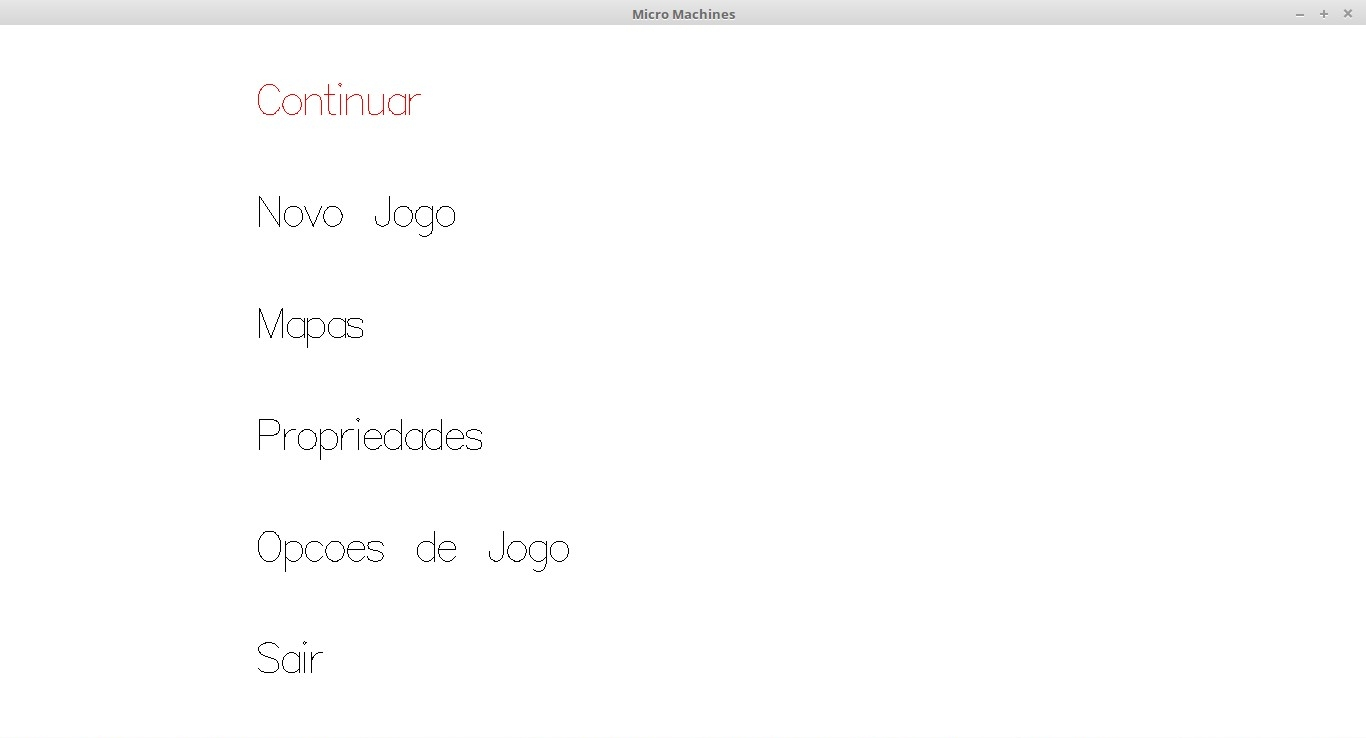
\includegraphics[scale=0.15]{foto.jpg}
\caption{Menu Principal}
\end{figure}


que é criado pelas funções drawMainMenu que devolve a imagem do menu principal e mainMenuOpts onde estão as opções contidas no menu principal.
Neste menu temos a opção de continuar o jogo, de iniciar um novo jogo e temos um menu de mapas, propriedades, opções de jogo assim como a opção de sair, que encerra o jogo.

O menu de mapas tem o seguinte aspeto :


\begin{figure}[!h]
\centering
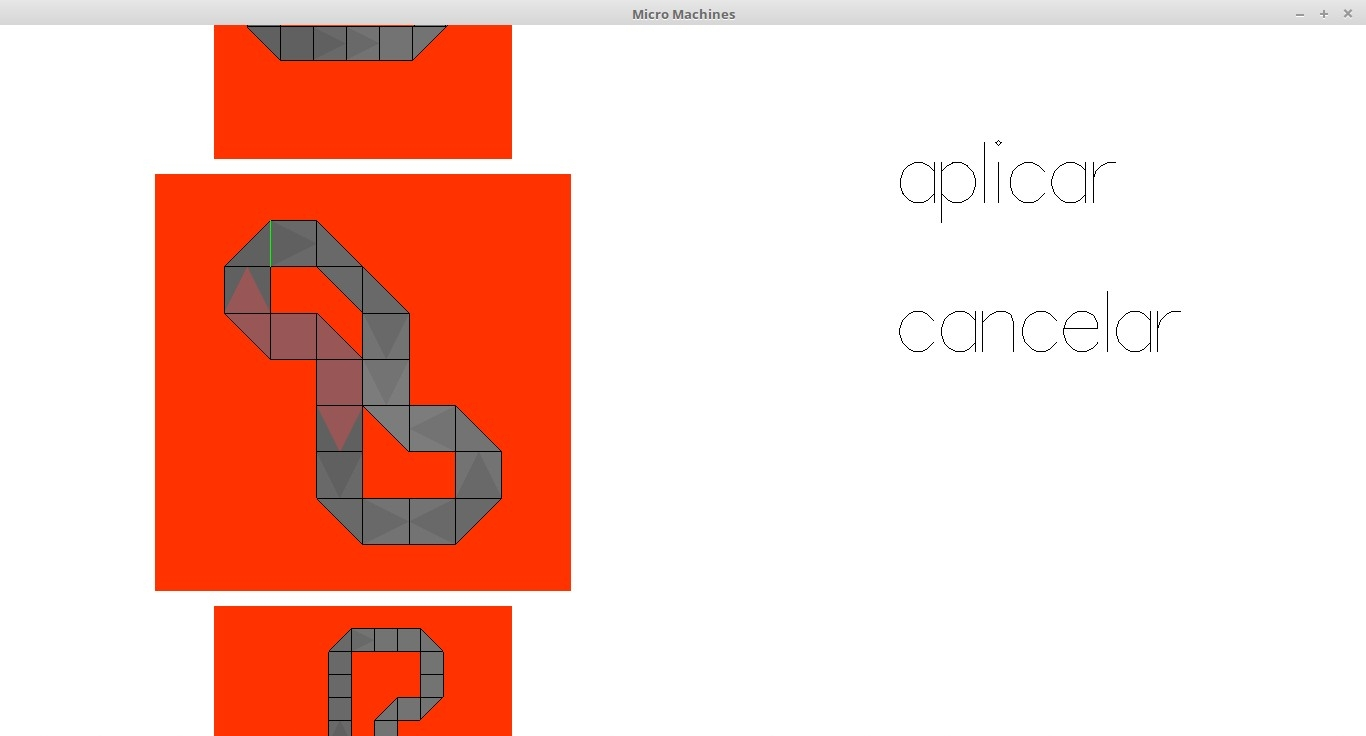
\includegraphics[scale=0.15]{foto(1).jpg}
\caption{Menu de Mapas}
\end{figure}


Neste menu é possível escolher qual o mapa que o utilizador pretende jogar.
O menu de mapas é controlado pela função setupMapSelection, que inicia o menu de seleção de mapas através do menu principal, a função drawMapSelectionMenuMaps, que devolve a imagem dos mapas no menu de seleção de mapas e a função drawOptsMapSelect, que devolve a imagem das opções no menu de seleção de mapas.


O menu de propriedades tem o seguinte aspeto :

\begin{figure}[!h]
\centering
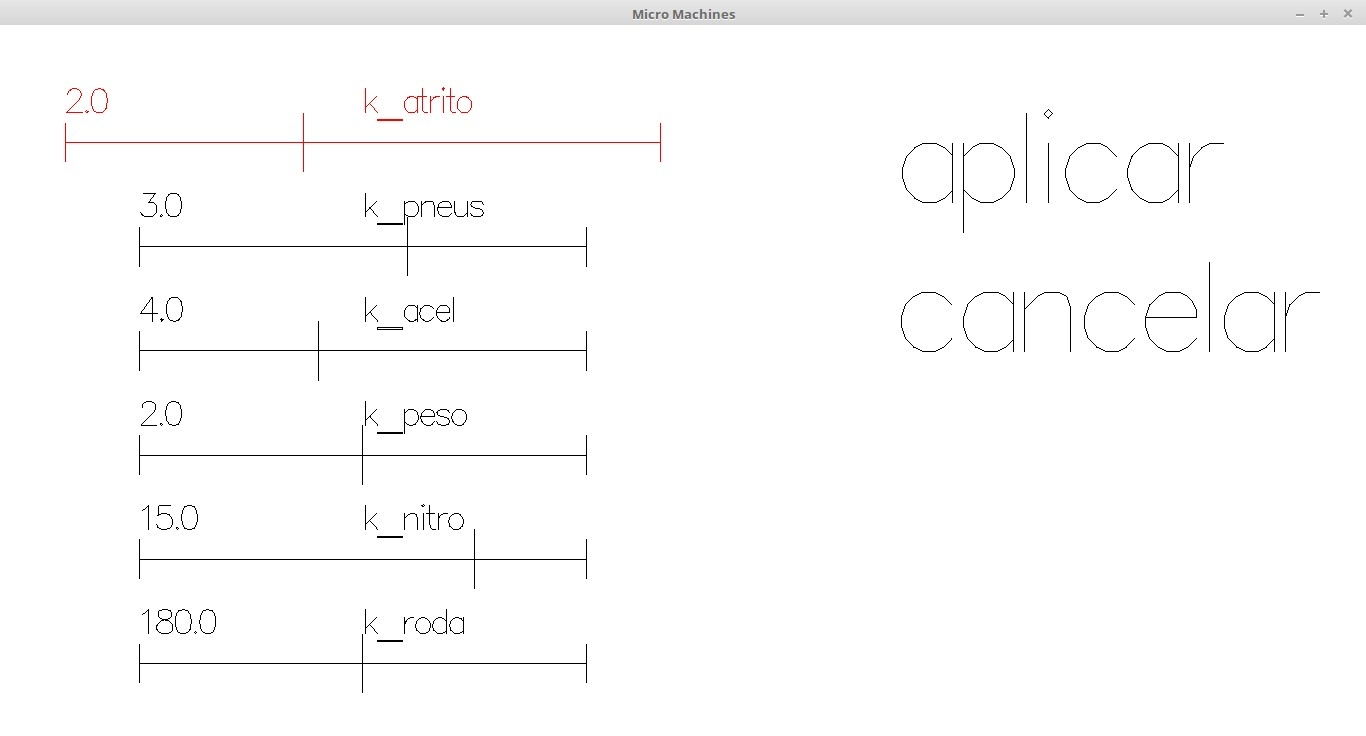
\includegraphics[scale=0.2]{foto(2).jpg}
\caption{Menu de Propriedades}
\end{figure}


Neste menu é possível alterar as propriedades do jogo, tais como, a força de atrito da pista, peso do carro etc.
Este menu é composto pela função toPropMenu que troca o estado de jogo de um menu principal para um menu de propriedades, a função menuToProps que extrai as propriedades contidas nos sliders de um Menu de propriedades e a função stringSliderProps que devolve uma lista de tuplos com os sliders iniciados relativamente às propriedades e a sua descrição correspondente.



O menu de opções de jogo tem o seguinte aspeto :

\begin{figure}[!h]
\centering
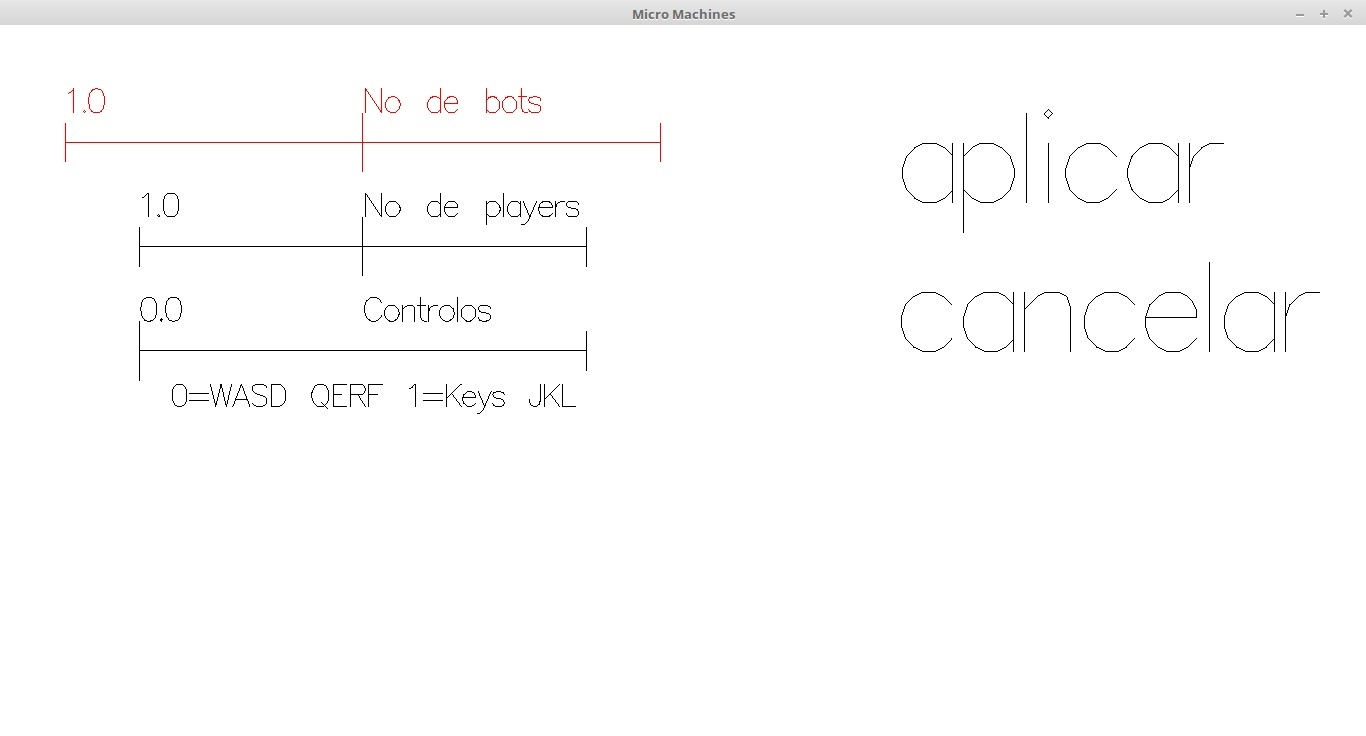
\includegraphics[scale=0.2]{foto(3).jpg}
\caption{Menu de Opções de Jogo}
\end{figure}


Neste menu é possível alterar o número de bots, o número de jogadores e o tipo de controlos do jogador.
Este menu é composto pela função toSettingsMenu, que troca o estado de jogo de um menu principal para um menu de opcoes de jogo, e onde a função stringSliderOpts devolve uma lista de tuplos com os sliders iniciados relativamente às propriedades e a sua descrição correspondente.É também composto pela função menuToSettings que extrai as opções contidas nos sliders do menu de opções.

Outras funções que criamos para esta subfase são a função setupNewGame que inicia um jogo novo através do menu principal, resetGame que reseta o jogo quando um dos carros ganha a corrida, resumeGame que volta ao jogo que estáva pausado anteriormente, updateActionBots que devolve a ação dos bots consoante o jogo, checkWonGame que testa se algum carro ganhou a partida e updateCarros que devolve os valores atualizados dos carros, nitros e históricos.


\subsection{Implementação de um Bot}

O objetivo desta subfase é a implementação de um bot que jogue micro machines automaticamente.
A solução que encontrámos para este problema é a função bot : 

\begin{verbatim}
bot :: Tempo  -- ^ tempo decorrido desde a última decisão
    -> Jogo   -- ^ estado atual do jogo
    -> Int    -- ^ identificador do jogador dentro do estado
    -> Acao   -- ^ a decisão tomada pelo /bot/
bot tick (Jogo mapa props carros _ hist) j 
  = (Acao acel trav dir esq useNitro)
  where
  myCar = carros !! j
  myHist = hist !! j
  percurso = definePercurso mapa
  target = desiredPos myCar myHist percurso
  (acel,trav,selfNitro) = acaoAcelerar myCar props target
  (dir,esq)   = steering myCar target --guiador' myCar target

  mainSelfNitro = selfNitroMapa myCar props mapa target  
  useNitro
    |nitroAdv /= Nothing = nitroAdv
    |mainSelfNitro = Just j
    |otherwise = Nothing

  nitroAdv = nitroAdversarios carros indexCarrosAFrente props mapa

  indexCarrosAFrente = aFrente lugares j
  lugares = getPosicoes indexs 
  indexs = getIndexs carros hist percurso

bot2 tick jogo j
  = (Acao acel trav dir esq Nothing)
  where
  (Acao acel trav dir esq _) = bot tick jogo j

\end{verbatim}
que é composta por várias outras funções como a função definePercurso que define um percurso através de um mapa, a função desiredPos :

\begin{verbatim}
desiredPos :: Carro -> [Posicao] -> Percurso -> Ponto
desiredPos (Carro (x,y) _ _) hist percurso
  = getDesiredPos index percurso
  where
  last3Pos = takeFirst 3 hist
  fPos = if hist == [] then (floor x, floor y)
         else hist !! 0
  percursos = partition fPos percurso
  ocurrenceIndex = mostElem last3Pos percursos
  index = searchPosIndex fPos percursoPos (ocurrenceIndex) 0
  (percursoPos,_,_) = unzip3 percurso
\end{verbatim}
que devolve a posição que o carro quer seguir e usa funções auxiliares como a função getDesiredPos que têm a mesma função mas recebe o indice de onde o carro se encontra na pista, a função searchPosIndex : 

\begin{verbatim}
searchPosIndex :: Posicao -> [Posicao] -> Int -> Int -> Int
searchPosIndex _ [] _ _ = 0
searchPosIndex pc (p:ps) i n
  = case (i,pc==p) of
    (_,False) -> searchPosIndex pc ps i (n+1)
    (0,True ) -> n
    otherwise -> searchPosIndex pc ps (i-1) (n+1)
\end{verbatim}
que procura o índice de uma posição numa lista de posições, e por último as funções takeFirst, partition e mostElem que retira os primeiros n elementos do inicio de uma lista, separa um percurso em partes em que uma certa posição se repete, devolve a parte do percurso que têm mais posições compatíveis com
uma lista de posições, respetivamente.

Uma outra função que compoê a função bot é a função acaoAcelarar :

\begin{verbatim}
acaoAcelerar :: Carro -> Propriedades -> Ponto -> (Bool,Bool,Bool)
acaoAcelerar (Carro pos ang vel) props desiredPos
  |vDot vAng vel < 0 = (True,False,True)
  |diff <  0 = (False,True ,False)
  |diff >  (desVel/1.5) = (True,False,True)
  |diff >  0 = (True ,False,False)
  |otherwise = (False,False,False)
  where
  posToDesired = vAdd desiredPos (vMult pos (-1))  
  mag = vMag vel
  vAng = vFromAngle ang
  desVel = if vDot posToDesired vAng < 0 then mag
           else desiredVel props
  diff = desVel - mag
\end{verbatim}
que controla se o carro está a acelerar ou a travar e usa como função auxiliar a função desiredPos, já falada anteriormente e a função desiredVel que devolve a velocidade desejada dependendo das propriedades da pista, assim como outras funções relacionadas com oprações de vetores da nossa libraria.

Na função bot é usada também a função steering : 

\begin{verbatim}
steering :: Carro -> Ponto -> (Bool,Bool)
steering (Carro a ang vel) c
  |turn > 0 = (False,True)
  |turn < 0 = (True,False)
  |turn ==0 = (False,False)
  where
  b = vAdd a (vFromAngle (vDegreeToRad (-ang)))
  (abx,aby) = vAdd b (vMult a (-1))
  (acx,acy) = vAdd c (vMult a (-1))
  vAB3D = (realToFrac abx,realToFrac aby,0)
  vAC3D = (realToFrac acx,realToFrac acy,0)
  (_,_,turn) = vCrossProduct3by3 vAB3D vAC3D
\end{verbatim}
que controla o guiador do carro e onde são usadas várias funções auxiliares da nossa libraria de vetores.

Para controlar o uso do nitro em si próprio, é usada na função bot a função selfNitroMapa :

\begin{verbatim}
selfNitroMapa :: Carro -> Propriedades -> Mapa -> Ponto -> Bool
selfNitroMapa (Carro pos@(x,y) a vel) (Propriedades atr _ _ _ _ _) (Mapa _ tab) desiredPos@(dx,dy)
  |vDot posToDesired vel < 0 = False
  |h<0 = True
  |h>=0= False
  where
  isCurva :: Tipo -> Bool
  isCurva (Curva _) = True
  isCurva _ = False

  angC = vAngleBetween (vFromAngle (vDegreeToRad (-a))) posToDesired
  angVel = vAngleBetween vel posToDesired

  posToDesired = vAdd desiredPos (vMult pos (-1)) 
  (Peca t h) = (tab !! (floor y)) !! (floor x)
  (Peca td _) = (tab !! (floor dy) !! floor dx)
\end{verbatim}
e para controlar situações onde o bot usa o nitro nos adversários é usada a função nitroAdv :

\begin{verbatim}
nitroAdversarios :: [Carro] -> [Int] -> Propriedades -> Mapa -> Maybe Int
nitroAdversarios [] _ _ _ = Nothing
nitroAdversarios _ [] _ _ = Nothing
nitroAdversarios carros (i:is) props@(Propriedades atr _ _ _ _ _) map@(Mapa _ tab)
  = case t of
    (Curva _) -> if h>=0 && atr <1 then Just i
                 else nitroAdversarios carros is props map
    otherwise -> nitroAdversarios carros is props map
  where
  (Carro (x,y) _ _) = carros !! i
  (fx,fy) = (floor x, floor y)
  (Peca t h) = (tab !! fy) !! fx
\end{verbatim}

Outras funções usadas na função bot são funções como a função aFrente que devolve os indices dos carros que estão à frente de um certo carro, a função getPosicoes que obtem os lugares em que os carros se encontram através do indice da peca da pista em que se encontram e a função getIndex que obtem as posições de todos os carros.


% Como foi validada a implementação da solução
\chapter{Validação da Solução}

Todas as fases excluindo as subfases 5 e 6 foram testadas no sistema de feedback disponibilizado pelos professores, e todos os testes estavam ok.
Quanto à subfase 5, o projeto foi testado pelos criadores e terceiros, pelo que concluímos que o jogo está jogável.
Por último, quanto à subfase 6 concluimos que o nosso bot está aceitável.


\chapter{Conclusão}

Conclui-se que todos os problemas que nos foram propostos foram bem executados. A nossa versão do jogo Micro Machines apresenta gráficos e menus aplativos.
Acrescentá-mos ainda que o jogo superou as nossas expectativas embora nos tenha aparecido no final um bug inexperado. Apesar de não ter-mos chegado à raiz do problema devido a falta de tempo, suspeitá-mos que o bug se trate de um caso especial na subfase 3 onde a função que retorna a nova velocidade do carro fica em loop infinito.

\end{document}
